\documentclass[1p]{elsarticle_modified}
%\bibliographystyle{elsarticle-num}

%\usepackage[colorlinks]{hyperref}
%\usepackage{abbrmath_seonhwa} %\Abb, \Ascr, \Acal ,\Abf, \Afrak
\usepackage{amsfonts}
\usepackage{amssymb}
\usepackage{amsmath}
\usepackage{amsthm}
\usepackage{scalefnt}
\usepackage{amsbsy}
\usepackage{kotex}
\usepackage{caption}
\usepackage{subfig}
\usepackage{color}
\usepackage{graphicx}
\usepackage{xcolor} %% white, black, red, green, blue, cyan, magenta, yellow
\usepackage{float}
\usepackage{setspace}
\usepackage{hyperref}

\usepackage{tikz}
\usetikzlibrary{arrows}

\usepackage{multirow}
\usepackage{array} % fixed length table
\usepackage{hhline}

%%%%%%%%%%%%%%%%%%%%%
\makeatletter
\renewcommand*\env@matrix[1][\arraystretch]{%
	\edef\arraystretch{#1}%
	\hskip -\arraycolsep
	\let\@ifnextchar\new@ifnextchar
	\array{*\c@MaxMatrixCols c}}
\makeatother %https://tex.stackexchange.com/questions/14071/how-can-i-increase-the-line-spacing-in-a-matrix
%%%%%%%%%%%%%%%

\usepackage[normalem]{ulem}

\newcommand{\msout}[1]{\ifmmode\text{\sout{\ensuremath{#1}}}\else\sout{#1}\fi}
%SOURCE: \msout is \stkout macro in https://tex.stackexchange.com/questions/20609/strikeout-in-math-mode

\newcommand{\cancel}[1]{
	\ifmmode
	{\color{red}\msout{#1}}
	\else
	{\color{red}\sout{#1}}
	\fi
}

\newcommand{\add}[1]{
	{\color{blue}\uwave{#1}}
}

\newcommand{\replace}[2]{
	\ifmmode
	{\color{red}\msout{#1}}{\color{blue}\uwave{#2}}
	\else
	{\color{red}\sout{#1}}{\color{blue}\uwave{#2}}
	\fi
}

\newcommand{\Sol}{\mathcal{S}} %segment
\newcommand{\D}{D} %diagram
\newcommand{\A}{\mathcal{A}} %arc


%%%%%%%%%%%%%%%%%%%%%%%%%%%%%5 test

\def\sl{\operatorname{\textup{SL}}(2,\Cbb)}
\def\psl{\operatorname{\textup{PSL}}(2,\Cbb)}
\def\quan{\mkern 1mu \triangleright \mkern 1mu}

\theoremstyle{definition}
\newtheorem{thm}{Theorem}[section]
\newtheorem{prop}[thm]{Proposition}
\newtheorem{lem}[thm]{Lemma}
\newtheorem{ques}[thm]{Question}
\newtheorem{cor}[thm]{Corollary}
\newtheorem{defn}[thm]{Definition}
\newtheorem{exam}[thm]{Example}
\newtheorem{rmk}[thm]{Remark}
\newtheorem{alg}[thm]{Algorithm}

\newcommand{\I}{\sqrt{-1}}
\begin{document}

%\begin{frontmatter}
%
%\title{Boundary parabolic representations of knots up to 8 crossings}
%
%%% Group authors per affiliation:
%\author{Yunhi Cho} 
%\address{Department of Mathematics, University of Seoul, Seoul, Korea}
%\ead{yhcho@uos.ac.kr}
%
%
%\author{Seonhwa Kim} %\fnref{s_kim}}
%\address{Center for Geometry and Physics, Institute for Basic Science, Pohang, 37673, Korea}
%\ead{ryeona17@ibs.re.kr}
%
%\author{Hyuk Kim}
%\address{Department of Mathematical Sciences, Seoul National University, Seoul 08826, Korea}
%\ead{hyukkim@snu.ac.kr}
%
%\author{Seokbeom Yoon}
%\address{Department of Mathematical Sciences, Seoul National University, Seoul, 08826,  Korea}
%\ead{sbyoon15@snu.ac.kr}
%
%\begin{abstract}
%We find all boundary parabolic representation of knots up to 8 crossings.
%
%\end{abstract}
%\begin{keyword}
%    \MSC[2010] 57M25 
%\end{keyword}
%
%\end{frontmatter}

%\linenumbers
%\tableofcontents
%
\newcommand\colored[1]{\textcolor{white}{\rule[-0.35ex]{0.8em}{1.4ex}}\kern-0.8em\color{red} #1}%
%\newcommand\colored[1]{\textcolor{white}{ #1}\kern-2.17ex	\textcolor{white}{ #1}\kern-1.81ex	\textcolor{white}{ #1}\kern-2.15ex\color{red}#1	}

{\Large $\underline{11a_{105}~(K11a_{105})}$}

\setlength{\tabcolsep}{10pt}
\renewcommand{\arraystretch}{1.6}
\vspace{1cm}\begin{tabular}{m{100pt}>{\centering\arraybackslash}m{274pt}}
\multirow{5}{120pt}{
	\centering
	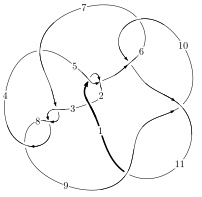
\includegraphics[width=112pt]{../../../GIT/diagram.site/Diagrams/png/354_11a_105.png}\\
\ \ \ A knot diagram\footnotemark}&
\allowdisplaybreaks
\textbf{Linearized knot diagam} \\
\cline{2-2}
 &
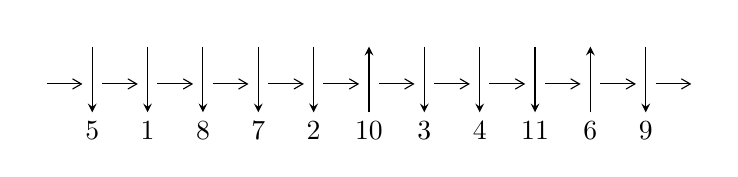
\begin{tikzpicture}[x=20pt, y=17pt]
	% nodes
	\node (C0) at (0, 0) {};
	\node (C1) at (1, 0) {};
	\node (C1U) at (1, +1) {};
	\node (C1D) at (1, -1) {5};

	\node (C2) at (2, 0) {};
	\node (C2U) at (2, +1) {};
	\node (C2D) at (2, -1) {1};

	\node (C3) at (3, 0) {};
	\node (C3U) at (3, +1) {};
	\node (C3D) at (3, -1) {8};

	\node (C4) at (4, 0) {};
	\node (C4U) at (4, +1) {};
	\node (C4D) at (4, -1) {7};

	\node (C5) at (5, 0) {};
	\node (C5U) at (5, +1) {};
	\node (C5D) at (5, -1) {2};

	\node (C6) at (6, 0) {};
	\node (C6U) at (6, +1) {};
	\node (C6D) at (6, -1) {10};

	\node (C7) at (7, 0) {};
	\node (C7U) at (7, +1) {};
	\node (C7D) at (7, -1) {3};

	\node (C8) at (8, 0) {};
	\node (C8U) at (8, +1) {};
	\node (C8D) at (8, -1) {4};

	\node (C9) at (9, 0) {};
	\node (C9U) at (9, +1) {};
	\node (C9D) at (9, -1) {11};

	\node (C10) at (10, 0) {};
	\node (C10U) at (10, +1) {};
	\node (C10D) at (10, -1) {6};

	\node (C11) at (11, 0) {};
	\node (C11U) at (11, +1) {};
	\node (C11D) at (11, -1) {9};
	\node (C12) at (12, 0) {};

	% arrows
	\draw[->,>={angle 60}]
	(C0) edge (C1) (C1) edge (C2) (C2) edge (C3) (C3) edge (C4) (C4) edge (C5) (C5) edge (C6) (C6) edge (C7) (C7) edge (C8) (C8) edge (C9) (C9) edge (C10) (C10) edge (C11) (C11) edge (C12) ;	\draw[->,>=stealth]
	(C1U) edge (C1D) (C2U) edge (C2D) (C3U) edge (C3D) (C4U) edge (C4D) (C5U) edge (C5D) (C6D) edge (C6U) (C7U) edge (C7D) (C8U) edge (C8D) (C9U) edge (C9D) (C10D) edge (C10U) (C11U) edge (C11D) ;
	\end{tikzpicture} \\
\hhline{~~} \\& 
\textbf{Solving Sequence} \\ \cline{2-2} 
 &
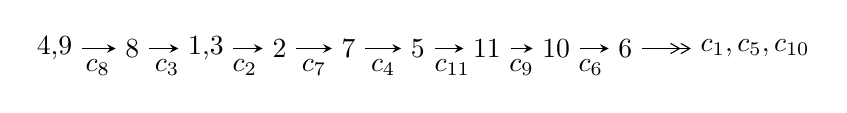
\begin{tikzpicture}[x=25pt, y=7pt]
	% node
	\node (A0) at (-1/8, 0) {4,9};
	\node (A1) at (1, 0) {8};
	\node (A2) at (33/16, 0) {1,3};
	\node (A3) at (25/8, 0) {2};
	\node (A4) at (33/8, 0) {7};
	\node (A5) at (41/8, 0) {5};
	\node (A6) at (49/8, 0) {11};
	\node (A7) at (57/8, 0) {10};
	\node (A8) at (65/8, 0) {6};
	\node (C1) at (1/2, -1) {$c_{8}$};
	\node (C2) at (3/2, -1) {$c_{3}$};
	\node (C3) at (21/8, -1) {$c_{2}$};
	\node (C4) at (29/8, -1) {$c_{7}$};
	\node (C5) at (37/8, -1) {$c_{4}$};
	\node (C6) at (45/8, -1) {$c_{11}$};
	\node (C7) at (53/8, -1) {$c_{9}$};
	\node (C8) at (61/8, -1) {$c_{6}$};
	\node (A9) at (10, 0) {$c_{1},c_{5},c_{10}$};

	% edge
	\draw[->,>=stealth]	
	(A0) edge (A1) (A1) edge (A2) (A2) edge (A3) (A3) edge (A4) (A4) edge (A5) (A5) edge (A6) (A6) edge (A7) (A7) edge (A8) ;
	\draw[->>,>={angle 60}]	
	(A8) edge (A9);
\end{tikzpicture} \\ 

\end{tabular} \\

\footnotetext{
The image of knot diagram is generated by the software ``\textbf{Draw programme}" developed by Andrew Bartholomew(\url{http://www.layer8.co.uk/maths/draw/index.htm\#Running-draw}), where we modified some parts for our purpose(\url{https://github.com/CATsTAILs/LinksPainter}).
}\phantom \\ \newline 
\centering \textbf{Ideals for irreducible components\footnotemark of $X_{\text{par}}$} 
 
\begin{align*}
I^u_{1}&=\langle 
1.12515\times10^{31} u^{59}+2.85842\times10^{31} u^{58}+\cdots+3.51410\times10^{31} b+1.89741\times10^{31},\\
\phantom{I^u_{1}}&\phantom{= \langle  }-3.51793\times10^{30} u^{59}-1.13761\times10^{31} u^{58}+\cdots+3.51410\times10^{31} a-1.05909\times10^{32},\;u^{60}+u^{59}+\cdots-4 u-4\rangle \\
I^u_{2}&=\langle 
2 b+2 a+u,\;2 a^2+2 a u+2 a+u+3,\;u^2-2\rangle \\
\\
I^v_{1}&=\langle 
a,\;b- v-1,\;v^2+v+1\rangle \\
\end{align*}
\raggedright * 3 irreducible components of $\dim_{\mathbb{C}}=0$, with total 66 representations.\\
\footnotetext{All coefficients of polynomials are rational numbers. But the coefficients are sometimes approximated in decimal forms when there is not enough margin.}
\newpage
\renewcommand{\arraystretch}{1}
\centering \section*{I. $I^u_{1}= \langle 1.13\times10^{31} u^{59}+2.86\times10^{31} u^{58}+\cdots+3.51\times10^{31} b+1.90\times10^{31},\;-3.52\times10^{30} u^{59}-1.14\times10^{31} u^{58}+\cdots+3.51\times10^{31} a-1.06\times10^{32},\;u^{60}+u^{59}+\cdots-4 u-4 \rangle$}
\flushleft \textbf{(i) Arc colorings}\\
\begin{tabular}{m{7pt} m{180pt} m{7pt} m{180pt} }
\flushright $a_{4}=$&$\begin{pmatrix}0\\u\end{pmatrix}$ \\
\flushright $a_{9}=$&$\begin{pmatrix}1\\0\end{pmatrix}$ \\
\flushright $a_{8}=$&$\begin{pmatrix}1\\- u^2\end{pmatrix}$ \\
\flushright $a_{1}=$&$\begin{pmatrix}0.100109 u^{59}+0.323727 u^{58}+\cdots+6.24684 u+3.01381\\-0.320182 u^{59}-0.813414 u^{58}+\cdots+3.67561 u-0.539941\end{pmatrix}$ \\
\flushright $a_{3}=$&$\begin{pmatrix}u\\- u^3+u\end{pmatrix}$ \\
\flushright $a_{2}=$&$\begin{pmatrix}0.334020 u^{59}+0.230566 u^{58}+\cdots+9.56791 u+3.49275\\-0.161128 u^{59}-0.574931 u^{58}+\cdots+3.42064 u-0.184944\end{pmatrix}$ \\
\flushright $a_{7}=$&$\begin{pmatrix}- u^2+1\\u^4-2 u^2\end{pmatrix}$ \\
\flushright $a_{5}=$&$\begin{pmatrix}- u^5+2 u^3- u\\u^7-3 u^5+2 u^3+u\end{pmatrix}$ \\
\flushright $a_{11}=$&$\begin{pmatrix}-0.220073 u^{59}-0.489687 u^{58}+\cdots+9.92245 u+2.47387\\-0.320182 u^{59}-0.813414 u^{58}+\cdots+3.67561 u-0.539941\end{pmatrix}$ \\
\flushright $a_{10}=$&$\begin{pmatrix}1.05972 u^{59}-0.120964 u^{58}+\cdots-11.8926 u-2.73515\\0.550795 u^{59}+1.41033 u^{58}+\cdots-3.83041 u+0.910068\end{pmatrix}$ \\
\flushright $a_{6}=$&$\begin{pmatrix}-0.301975 u^{59}-0.154593 u^{58}+\cdots-8.20559 u-4.09227\\0.609330 u^{59}+0.192047 u^{58}+\cdots+2.33523 u-2.20792\end{pmatrix}$\\ \flushright $a_{6}=$&$\begin{pmatrix}-0.301975 u^{59}-0.154593 u^{58}+\cdots-8.20559 u-4.09227\\0.609330 u^{59}+0.192047 u^{58}+\cdots+2.33523 u-2.20792\end{pmatrix}$\\&\end{tabular}
\flushleft \textbf{(ii) Obstruction class $= -1$}\\~\\
\flushleft \textbf{(iii) Cusp Shapes $= 1.29031 u^{59}+4.98190 u^{58}+\cdots+10.5616 u+3.04276$}\\~\\
\newpage\renewcommand{\arraystretch}{1}
\flushleft \textbf{(iv) u-Polynomials at the component}\newline \\
\begin{tabular}{m{50pt}|m{274pt}}
Crossings & \hspace{64pt}u-Polynomials at each crossing \\
\hline $$\begin{aligned}c_{1},c_{5}\end{aligned}$$&$\begin{aligned}
&u^{60}+3 u^{59}+\cdots-21 u-7
\end{aligned}$\\
\hline $$\begin{aligned}c_{2}\end{aligned}$$&$\begin{aligned}
&u^{60}+29 u^{59}+\cdots+259 u+49
\end{aligned}$\\
\hline $$\begin{aligned}c_{3},c_{7},c_{8}\end{aligned}$$&$\begin{aligned}
&u^{60}+u^{59}+\cdots-4 u-4
\end{aligned}$\\
\hline $$\begin{aligned}c_{4}\end{aligned}$$&$\begin{aligned}
&u^{60}-3 u^{59}+\cdots+1892 u+748
\end{aligned}$\\
\hline $$\begin{aligned}c_{6},c_{10}\end{aligned}$$&$\begin{aligned}
&u^{60}-2 u^{59}+\cdots+10 u+1
\end{aligned}$\\
\hline $$\begin{aligned}c_{9},c_{11}\end{aligned}$$&$\begin{aligned}
&u^{60}+20 u^{59}+\cdots-58 u+1
\end{aligned}$\\
\hline
\end{tabular}\\~\\
\newpage\renewcommand{\arraystretch}{1}
\flushleft \textbf{(v) Riley Polynomials at the component}\newline \\
\begin{tabular}{m{50pt}|m{274pt}}
Crossings & \hspace{64pt}Riley Polynomials at each crossing \\
\hline $$\begin{aligned}c_{1},c_{5}\end{aligned}$$&$\begin{aligned}
&y^{60}-29 y^{59}+\cdots-259 y+49
\end{aligned}$\\
\hline $$\begin{aligned}c_{2}\end{aligned}$$&$\begin{aligned}
&y^{60}+11 y^{59}+\cdots-38171 y+2401
\end{aligned}$\\
\hline $$\begin{aligned}c_{3},c_{7},c_{8}\end{aligned}$$&$\begin{aligned}
&y^{60}-55 y^{59}+\cdots+144 y+16
\end{aligned}$\\
\hline $$\begin{aligned}c_{4}\end{aligned}$$&$\begin{aligned}
&y^{60}+5 y^{59}+\cdots-713328 y+559504
\end{aligned}$\\
\hline $$\begin{aligned}c_{6},c_{10}\end{aligned}$$&$\begin{aligned}
&y^{60}+20 y^{59}+\cdots-58 y+1
\end{aligned}$\\
\hline $$\begin{aligned}c_{9},c_{11}\end{aligned}$$&$\begin{aligned}
&y^{60}+44 y^{59}+\cdots-3138 y+1
\end{aligned}$\\
\hline
\end{tabular}\\~\\
\newpage\flushleft \textbf{(vi) Complex Volumes and Cusp Shapes}
$$\begin{array}{c|c|c}  
\text{Solutions to }I^u_{1}& \I (\text{vol} + \sqrt{-1}CS) & \text{Cusp shape}\\
 \hline 
\begin{aligned}
u &= -0.856412 + 0.448917 I \\
a &= \phantom{-}0.069748 - 0.309881 I \\
b &= \phantom{-}0.045178 + 1.220370 I\end{aligned}
 & \phantom{-}2.51877 - 0.25684 I & -5.58857 - 0.91280 I \\ \hline\begin{aligned}
u &= -0.856412 - 0.448917 I \\
a &= \phantom{-}0.069748 + 0.309881 I \\
b &= \phantom{-}0.045178 - 1.220370 I\end{aligned}
 & \phantom{-}2.51877 + 0.25684 I & -5.58857 + 0.91280 I \\ \hline\begin{aligned}
u &= -0.977737 + 0.387234 I \\
a &= -0.646202 + 0.329883 I \\
b &= -0.199913 - 1.371860 I\end{aligned}
 & \phantom{-}2.99290 - 0.67802 I & -7.00000 + 0. I\phantom{ +0.000000I} \\ \hline\begin{aligned}
u &= -0.977737 - 0.387234 I \\
a &= -0.646202 - 0.329883 I \\
b &= -0.199913 + 1.371860 I\end{aligned}
 & \phantom{-}2.99290 + 0.67802 I & -7.00000 + 0. I\phantom{ +0.000000I} \\ \hline\begin{aligned}
u &= \phantom{-}0.791019 + 0.508592 I \\
a &= -0.325990 - 0.504077 I \\
b &= -0.39274 + 1.43077 I\end{aligned}
 & \phantom{-}1.89650 + 6.03755 I & -6.88192 - 4.20349 I \\ \hline\begin{aligned}
u &= \phantom{-}0.791019 - 0.508592 I \\
a &= -0.325990 + 0.504077 I \\
b &= -0.39274 - 1.43077 I\end{aligned}
 & \phantom{-}1.89650 - 6.03755 I & -6.88192 + 4.20349 I \\ \hline\begin{aligned}
u &= \phantom{-}1.068800 + 0.379471 I \\
a &= \phantom{-}0.494885 + 0.197200 I \\
b &= -0.116006 - 1.361990 I\end{aligned}
 & \phantom{-}3.09128 - 5.18590 I & \phantom{-0.000000 } 0 \\ \hline\begin{aligned}
u &= \phantom{-}1.068800 - 0.379471 I \\
a &= \phantom{-}0.494885 - 0.197200 I \\
b &= -0.116006 + 1.361990 I\end{aligned}
 & \phantom{-}3.09128 + 5.18590 I & \phantom{-0.000000 } 0 \\ \hline\begin{aligned}
u &= \phantom{-}0.301071 + 0.803639 I \\
a &= \phantom{-}1.174960 - 0.782603 I \\
b &= -0.48181 - 1.50728 I\end{aligned}
 & \phantom{-}3.49971 - 10.62980 I & -5.43356 + 8.51745 I \\ \hline\begin{aligned}
u &= \phantom{-}0.301071 - 0.803639 I \\
a &= \phantom{-}1.174960 + 0.782603 I \\
b &= -0.48181 + 1.50728 I\end{aligned}
 & \phantom{-}3.49971 + 10.62980 I & -5.43356 - 8.51745 I\\
 \hline 
 \end{array}$$\newpage$$\begin{array}{c|c|c}  
\text{Solutions to }I^u_{1}& \I (\text{vol} + \sqrt{-1}CS) & \text{Cusp shape}\\
 \hline 
\begin{aligned}
u &= -0.256488 + 0.801752 I \\
a &= -1.204450 - 0.589990 I \\
b &= \phantom{-}0.206818 - 1.186610 I\end{aligned}
 & \phantom{-}4.44819 + 4.71708 I & -3.57538 - 3.65619 I \\ \hline\begin{aligned}
u &= -0.256488 - 0.801752 I \\
a &= -1.204450 + 0.589990 I \\
b &= \phantom{-}0.206818 + 1.186610 I\end{aligned}
 & \phantom{-}4.44819 - 4.71708 I & -3.57538 + 3.65619 I \\ \hline\begin{aligned}
u &= -0.189775 + 0.793215 I \\
a &= \phantom{-}0.692391 + 1.041360 I \\
b &= -0.34795 + 1.45648 I\end{aligned}
 & \phantom{-}5.43709 + 4.96254 I & -2.32735 - 3.96471 I \\ \hline\begin{aligned}
u &= -0.189775 - 0.793215 I \\
a &= \phantom{-}0.692391 - 1.041360 I \\
b &= -0.34795 - 1.45648 I\end{aligned}
 & \phantom{-}5.43709 - 4.96254 I & -2.32735 + 3.96471 I \\ \hline\begin{aligned}
u &= \phantom{-}0.129554 + 0.796054 I \\
a &= -0.844160 + 0.874550 I \\
b &= \phantom{-}0.043508 + 1.278600 I\end{aligned}
 & \phantom{-}5.97615 + 0.93056 I & -1.28101 - 1.70769 I \\ \hline\begin{aligned}
u &= \phantom{-}0.129554 - 0.796054 I \\
a &= -0.844160 - 0.874550 I \\
b &= \phantom{-}0.043508 - 1.278600 I\end{aligned}
 & \phantom{-}5.97615 - 0.93056 I & -1.28101 + 1.70769 I \\ \hline\begin{aligned}
u &= -1.206730 + 0.176348 I \\
a &= -1.133230 - 0.267587 I \\
b &= \phantom{-}0.418519 + 0.150611 I\end{aligned}
 & -1.73220 + 0.82680 I & \phantom{-0.000000 } 0 \\ \hline\begin{aligned}
u &= -1.206730 - 0.176348 I \\
a &= -1.133230 + 0.267587 I \\
b &= \phantom{-}0.418519 - 0.150611 I\end{aligned}
 & -1.73220 - 0.82680 I & \phantom{-0.000000 } 0 \\ \hline\begin{aligned}
u &= \phantom{-}1.243970 + 0.018853 I \\
a &= \phantom{-}1.26750 - 0.88605 I \\
b &= -0.868501 + 0.830940 I\end{aligned}
 & -4.34425 + 2.84333 I & \phantom{-0.000000 } 0 \\ \hline\begin{aligned}
u &= \phantom{-}1.243970 - 0.018853 I \\
a &= \phantom{-}1.26750 + 0.88605 I \\
b &= -0.868501 - 0.830940 I\end{aligned}
 & -4.34425 - 2.84333 I & \phantom{-0.000000 } 0\\
 \hline 
 \end{array}$$\newpage$$\begin{array}{c|c|c}  
\text{Solutions to }I^u_{1}& \I (\text{vol} + \sqrt{-1}CS) & \text{Cusp shape}\\
 \hline 
\begin{aligned}
u &= \phantom{-}0.268078 + 0.645087 I \\
a &= \phantom{-}0.627642 - 0.518062 I \\
b &= -1.102390 - 0.396751 I\end{aligned}
 & -2.44529 - 4.90792 I & -9.88732 + 7.39777 I \\ \hline\begin{aligned}
u &= \phantom{-}0.268078 - 0.645087 I \\
a &= \phantom{-}0.627642 + 0.518062 I \\
b &= -1.102390 + 0.396751 I\end{aligned}
 & -2.44529 + 4.90792 I & -9.88732 - 7.39777 I \\ \hline\begin{aligned}
u &= \phantom{-}1.289880 + 0.180120 I \\
a &= -1.66882 + 0.29795 I \\
b &= -0.038165 + 1.051040 I\end{aligned}
 & -4.50001 - 0.00587 I & \phantom{-0.000000 } 0 \\ \hline\begin{aligned}
u &= \phantom{-}1.289880 - 0.180120 I \\
a &= -1.66882 - 0.29795 I \\
b &= -0.038165 - 1.051040 I\end{aligned}
 & -4.50001 + 0.00587 I & \phantom{-0.000000 } 0 \\ \hline\begin{aligned}
u &= -0.112152 + 0.661191 I \\
a &= -0.714620 - 0.045202 I \\
b &= \phantom{-}0.426053 + 0.174796 I\end{aligned}
 & \phantom{-}1.43580 + 2.21650 I & -1.82720 - 4.33305 I \\ \hline\begin{aligned}
u &= -0.112152 - 0.661191 I \\
a &= -0.714620 + 0.045202 I \\
b &= \phantom{-}0.426053 - 0.174796 I\end{aligned}
 & \phantom{-}1.43580 - 2.21650 I & -1.82720 + 4.33305 I \\ \hline\begin{aligned}
u &= -1.334650 + 0.196412 I \\
a &= \phantom{-}1.04014 + 1.40007 I \\
b &= -0.877556 - 1.103860 I\end{aligned}
 & -5.48660 + 1.01058 I & \phantom{-0.000000 } 0 \\ \hline\begin{aligned}
u &= -1.334650 - 0.196412 I \\
a &= \phantom{-}1.04014 - 1.40007 I \\
b &= -0.877556 + 1.103860 I\end{aligned}
 & -5.48660 - 1.01058 I & \phantom{-0.000000 } 0 \\ \hline\begin{aligned}
u &= -1.333660 + 0.221254 I \\
a &= \phantom{-}1.82839 + 0.49243 I \\
b &= -0.448347 + 1.321910 I\end{aligned}
 & -5.17207 + 5.38877 I & \phantom{-0.000000 } 0 \\ \hline\begin{aligned}
u &= -1.333660 - 0.221254 I \\
a &= \phantom{-}1.82839 - 0.49243 I \\
b &= -0.448347 - 1.321910 I\end{aligned}
 & -5.17207 - 5.38877 I & \phantom{-0.000000 } 0\\
 \hline 
 \end{array}$$\newpage$$\begin{array}{c|c|c}  
\text{Solutions to }I^u_{1}& \I (\text{vol} + \sqrt{-1}CS) & \text{Cusp shape}\\
 \hline 
\begin{aligned}
u &= \phantom{-}1.331350 + 0.263582 I \\
a &= -1.077490 + 0.564419 I \\
b &= \phantom{-}0.496619 - 0.385771 I\end{aligned}
 & -3.10541 - 5.57944 I & \phantom{-0.000000 } 0 \\ \hline\begin{aligned}
u &= \phantom{-}1.331350 - 0.263582 I \\
a &= -1.077490 - 0.564419 I \\
b &= \phantom{-}0.496619 + 0.385771 I\end{aligned}
 & -3.10541 + 5.57944 I & \phantom{-0.000000 } 0 \\ \hline\begin{aligned}
u &= \phantom{-}1.352790 + 0.191832 I \\
a &= \phantom{-}1.57075 - 0.21221 I \\
b &= -1.044160 - 0.411993 I\end{aligned}
 & -5.42970 - 3.53470 I & \phantom{-0.000000 } 0 \\ \hline\begin{aligned}
u &= \phantom{-}1.352790 - 0.191832 I \\
a &= \phantom{-}1.57075 + 0.21221 I \\
b &= -1.044160 + 0.411993 I\end{aligned}
 & -5.42970 + 3.53470 I & \phantom{-0.000000 } 0 \\ \hline\begin{aligned}
u &= -1.334670 + 0.330501 I \\
a &= -1.55791 + 0.32540 I \\
b &= \phantom{-}0.175954 - 1.190020 I\end{aligned}
 & \phantom{-}1.38298 + 3.12184 I & \phantom{-0.000000 } 0 \\ \hline\begin{aligned}
u &= -1.334670 - 0.330501 I \\
a &= -1.55791 - 0.32540 I \\
b &= \phantom{-}0.175954 + 1.190020 I\end{aligned}
 & \phantom{-}1.38298 - 3.12184 I & \phantom{-0.000000 } 0 \\ \hline\begin{aligned}
u &= \phantom{-}0.461911 + 0.406202 I \\
a &= \phantom{-}0.28123 - 1.64366 I \\
b &= -0.821473 + 0.229272 I\end{aligned}
 & -3.41083 + 1.56394 I & -13.77106 - 0.02572 I \\ \hline\begin{aligned}
u &= \phantom{-}0.461911 - 0.406202 I \\
a &= \phantom{-}0.28123 + 1.64366 I \\
b &= -0.821473 - 0.229272 I\end{aligned}
 & -3.41083 - 1.56394 I & -13.77106 + 0.02572 I \\ \hline\begin{aligned}
u &= \phantom{-}1.38882\phantom{ +0.000000I} \\
a &= -0.894922\phantom{ +0.000000I} \\
b &= \phantom{-}0.0181684\phantom{ +0.000000I}\end{aligned}
 & -6.53287\phantom{ +0.000000I} & \phantom{-0.000000 } 0 \\ \hline\begin{aligned}
u &= \phantom{-}1.373810 + 0.327896 I \\
a &= \phantom{-}1.74591 + 0.30759 I \\
b &= -0.46361 - 1.49242 I\end{aligned}
 & \phantom{-}0.49565 - 9.00597 I & \phantom{-0.000000 } 0\\
 \hline 
 \end{array}$$\newpage$$\begin{array}{c|c|c}  
\text{Solutions to }I^u_{1}& \I (\text{vol} + \sqrt{-1}CS) & \text{Cusp shape}\\
 \hline 
\begin{aligned}
u &= \phantom{-}1.373810 - 0.327896 I \\
a &= \phantom{-}1.74591 - 0.30759 I \\
b &= -0.46361 + 1.49242 I\end{aligned}
 & \phantom{-}0.49565 + 9.00597 I & \phantom{-0.000000 } 0 \\ \hline\begin{aligned}
u &= -1.40111 + 0.26118 I \\
a &= \phantom{-}1.94947 + 0.43052 I \\
b &= -1.259340 + 0.325492 I\end{aligned}
 & -7.75888 + 8.23897 I & \phantom{-0.000000 } 0 \\ \hline\begin{aligned}
u &= -1.40111 - 0.26118 I \\
a &= \phantom{-}1.94947 - 0.43052 I \\
b &= -1.259340 - 0.325492 I\end{aligned}
 & -7.75888 - 8.23897 I & \phantom{-0.000000 } 0 \\ \hline\begin{aligned}
u &= \phantom{-}0.071840 + 0.552974 I \\
a &= \phantom{-}0.01528 - 3.02987 I \\
b &= -0.330288 - 1.143560 I\end{aligned}
 & -0.69378 - 2.54574 I & -3.93469 + 4.38996 I \\ \hline\begin{aligned}
u &= \phantom{-}0.071840 - 0.552974 I \\
a &= \phantom{-}0.01528 + 3.02987 I \\
b &= -0.330288 + 1.143560 I\end{aligned}
 & -0.69378 + 2.54574 I & -3.93469 - 4.38996 I \\ \hline\begin{aligned}
u &= -1.43987 + 0.14560 I \\
a &= \phantom{-}1.24613 + 0.98490 I \\
b &= -0.917886 + 0.053868 I\end{aligned}
 & -9.46417 + 0.48874 I & \phantom{-0.000000 } 0 \\ \hline\begin{aligned}
u &= -1.43987 - 0.14560 I \\
a &= \phantom{-}1.24613 - 0.98490 I \\
b &= -0.917886 - 0.053868 I\end{aligned}
 & -9.46417 - 0.48874 I & \phantom{-0.000000 } 0 \\ \hline\begin{aligned}
u &= \phantom{-}1.41119 + 0.32817 I \\
a &= -1.73533 - 0.42501 I \\
b &= \phantom{-}0.304129 + 1.125510 I\end{aligned}
 & -0.85298 - 8.80531 I & \phantom{-0.000000 } 0 \\ \hline\begin{aligned}
u &= \phantom{-}1.41119 - 0.32817 I \\
a &= -1.73533 + 0.42501 I \\
b &= \phantom{-}0.304129 - 1.125510 I\end{aligned}
 & -0.85298 + 8.80531 I & \phantom{-0.000000 } 0 \\ \hline\begin{aligned}
u &= -1.43461 + 0.32355 I \\
a &= \phantom{-}2.01968 - 0.51742 I \\
b &= -0.55973 + 1.52348 I\end{aligned}
 & -2.0394 + 14.7170 I & \phantom{-0.000000 } 0\\
 \hline 
 \end{array}$$\newpage$$\begin{array}{c|c|c}  
\text{Solutions to }I^u_{1}& \I (\text{vol} + \sqrt{-1}CS) & \text{Cusp shape}\\
 \hline 
\begin{aligned}
u &= -1.43461 - 0.32355 I \\
a &= \phantom{-}2.01968 + 0.51742 I \\
b &= -0.55973 - 1.52348 I\end{aligned}
 & -2.0394 - 14.7170 I & \phantom{-0.000000 } 0 \\ \hline\begin{aligned}
u &= -0.263721 + 0.414290 I \\
a &= -0.089083 + 0.498277 I \\
b &= -0.547343 + 0.345848 I\end{aligned}
 & -0.480323 + 1.226230 I & -5.70379 - 5.33805 I \\ \hline\begin{aligned}
u &= -0.263721 - 0.414290 I \\
a &= -0.089083 - 0.498277 I \\
b &= -0.547343 - 0.345848 I\end{aligned}
 & -0.480323 - 1.226230 I & -5.70379 + 5.33805 I \\ \hline\begin{aligned}
u &= \phantom{-}1.51224 + 0.04246 I \\
a &= -0.021792 + 1.121390 I \\
b &= -0.159960 - 1.012480 I\end{aligned}
 & -5.24444 - 0.82507 I & \phantom{-0.000000 } 0 \\ \hline\begin{aligned}
u &= \phantom{-}1.51224 - 0.04246 I \\
a &= -0.021792 - 1.121390 I \\
b &= -0.159960 + 1.012480 I\end{aligned}
 & -5.24444 + 0.82507 I & \phantom{-0.000000 } 0 \\ \hline\begin{aligned}
u &= \phantom{-}0.085208 + 0.469629 I \\
a &= \phantom{-}0.229268 - 0.034778 I \\
b &= -0.760151 + 0.894401 I\end{aligned}
 & -0.97414 + 1.49816 I & -3.90867 + 1.16289 I \\ \hline\begin{aligned}
u &= \phantom{-}0.085208 - 0.469629 I \\
a &= \phantom{-}0.229268 + 0.034778 I \\
b &= -0.760151 - 0.894401 I\end{aligned}
 & -0.97414 - 1.49816 I & -3.90867 - 1.16289 I \\ \hline\begin{aligned}
u &= -1.52569 + 0.08141 I \\
a &= \phantom{-}0.37288 + 1.45493 I \\
b &= -0.438151 - 1.250040 I\end{aligned}
 & -5.76976 - 4.33338 I & \phantom{-0.000000 } 0 \\ \hline\begin{aligned}
u &= -1.52569 - 0.08141 I \\
a &= \phantom{-}0.37288 - 1.45493 I \\
b &= -0.438151 + 1.250040 I\end{aligned}
 & -5.76976 + 4.33338 I & \phantom{-0.000000 } 0 \\ \hline\begin{aligned}
u &= -0.439722\phantom{ +0.000000I} \\
a &= -1.31943\phantom{ +0.000000I} \\
b &= \phantom{-}0.0992099\phantom{ +0.000000I}\end{aligned}
 & -0.965483\phantom{ +0.000000I} & -10.6880\phantom{ +0.000000I}\\
 \hline 
 \end{array}$$\newpage\newpage\renewcommand{\arraystretch}{1}
\centering \section*{II. $I^u_{2}= \langle 2 b+2 a+u,\;2 a^2+2 a u+2 a+u+3,\;u^2-2 \rangle$}
\flushleft \textbf{(i) Arc colorings}\\
\begin{tabular}{m{7pt} m{180pt} m{7pt} m{180pt} }
\flushright $a_{4}=$&$\begin{pmatrix}0\\u\end{pmatrix}$ \\
\flushright $a_{9}=$&$\begin{pmatrix}1\\0\end{pmatrix}$ \\
\flushright $a_{8}=$&$\begin{pmatrix}1\\-2\end{pmatrix}$ \\
\flushright $a_{1}=$&$\begin{pmatrix}a\\- a-\frac{1}{2} u\end{pmatrix}$ \\
\flushright $a_{3}=$&$\begin{pmatrix}u\\- u\end{pmatrix}$ \\
\flushright $a_{2}=$&$\begin{pmatrix}a+u\\- a-\frac{3}{2} u\end{pmatrix}$ \\
\flushright $a_{7}=$&$\begin{pmatrix}-1\\0\end{pmatrix}$ \\
\flushright $a_{5}=$&$\begin{pmatrix}- u\\u\end{pmatrix}$ \\
\flushright $a_{11}=$&$\begin{pmatrix}-\frac{1}{2} u\\- a-\frac{1}{2} u\end{pmatrix}$ \\
\flushright $a_{10}=$&$\begin{pmatrix}\frac{1}{2} a u+\frac{3}{2}\\- a-\frac{1}{2} u-1\end{pmatrix}$ \\
\flushright $a_{6}=$&$\begin{pmatrix}a\\- a-\frac{1}{2} u\end{pmatrix}$\\ \flushright $a_{6}=$&$\begin{pmatrix}a\\- a-\frac{1}{2} u\end{pmatrix}$\\&\end{tabular}
\flushleft \textbf{(ii) Obstruction class $= 1$}\\~\\
\flushleft \textbf{(iii) Cusp Shapes $= -4 a-2 u-16$}\\~\\
\newpage\renewcommand{\arraystretch}{1}
\flushleft \textbf{(iv) u-Polynomials at the component}\newline \\
\begin{tabular}{m{50pt}|m{274pt}}
Crossings & \hspace{64pt}u-Polynomials at each crossing \\
\hline $$\begin{aligned}c_{1},c_{2}\end{aligned}$$&$\begin{aligned}
&(u+1)^4
\end{aligned}$\\
\hline $$\begin{aligned}c_{3},c_{4},c_{7}\\c_{8}\end{aligned}$$&$\begin{aligned}
&(u^2-2)^2
\end{aligned}$\\
\hline $$\begin{aligned}c_{5}\end{aligned}$$&$\begin{aligned}
&(u-1)^4
\end{aligned}$\\
\hline $$\begin{aligned}c_{6},c_{9}\end{aligned}$$&$\begin{aligned}
&(u^2- u+1)^2
\end{aligned}$\\
\hline $$\begin{aligned}c_{10},c_{11}\end{aligned}$$&$\begin{aligned}
&(u^2+u+1)^2
\end{aligned}$\\
\hline
\end{tabular}\\~\\
\newpage\renewcommand{\arraystretch}{1}
\flushleft \textbf{(v) Riley Polynomials at the component}\newline \\
\begin{tabular}{m{50pt}|m{274pt}}
Crossings & \hspace{64pt}Riley Polynomials at each crossing \\
\hline $$\begin{aligned}c_{1},c_{2},c_{5}\end{aligned}$$&$\begin{aligned}
&(y-1)^4
\end{aligned}$\\
\hline $$\begin{aligned}c_{3},c_{4},c_{7}\\c_{8}\end{aligned}$$&$\begin{aligned}
&(y-2)^4
\end{aligned}$\\
\hline $$\begin{aligned}c_{6},c_{9},c_{10}\\c_{11}\end{aligned}$$&$\begin{aligned}
&(y^2+y+1)^2
\end{aligned}$\\
\hline
\end{tabular}\\~\\
\newpage\flushleft \textbf{(vi) Complex Volumes and Cusp Shapes}
$$\begin{array}{c|c|c}  
\text{Solutions to }I^u_{2}& \I (\text{vol} + \sqrt{-1}CS) & \text{Cusp shape}\\
 \hline 
\begin{aligned}
u &= \phantom{-}1.41421\phantom{ +0.000000I} \\
a &= -1.20711 + 0.86603 I \\
b &= \phantom{-}0.500000 - 0.866025 I\end{aligned}
 & -6.57974 + 2.02988 I & -14.0000 - 3.4641 I \\ \hline\begin{aligned}
u &= \phantom{-}1.41421\phantom{ +0.000000I} \\
a &= -1.20711 - 0.86603 I \\
b &= \phantom{-}0.500000 + 0.866025 I\end{aligned}
 & -6.57974 - 2.02988 I & -14.0000 + 3.4641 I \\ \hline\begin{aligned}
u &= -1.41421\phantom{ +0.000000I} \\
a &= \phantom{-}0.207107 + 0.866025 I \\
b &= \phantom{-}0.500000 - 0.866025 I\end{aligned}
 & -6.57974 + 2.02988 I & -14.0000 - 3.4641 I \\ \hline\begin{aligned}
u &= -1.41421\phantom{ +0.000000I} \\
a &= \phantom{-}0.207107 - 0.866025 I \\
b &= \phantom{-}0.500000 + 0.866025 I\end{aligned}
 & -6.57974 - 2.02988 I & -14.0000 + 3.4641 I\\
 \hline 
 \end{array}$$\newpage\newpage\renewcommand{\arraystretch}{1}
\centering \section*{III. $I^v_{1}= \langle a,\;b- v-1,\;v^2+v+1 \rangle$}
\flushleft \textbf{(i) Arc colorings}\\
\begin{tabular}{m{7pt} m{180pt} m{7pt} m{180pt} }
\flushright $a_{4}=$&$\begin{pmatrix}v\\0\end{pmatrix}$ \\
\flushright $a_{9}=$&$\begin{pmatrix}1\\0\end{pmatrix}$ \\
\flushright $a_{8}=$&$\begin{pmatrix}1\\0\end{pmatrix}$ \\
\flushright $a_{1}=$&$\begin{pmatrix}0\\v+1\end{pmatrix}$ \\
\flushright $a_{3}=$&$\begin{pmatrix}v\\0\end{pmatrix}$ \\
\flushright $a_{2}=$&$\begin{pmatrix}v\\v+1\end{pmatrix}$ \\
\flushright $a_{7}=$&$\begin{pmatrix}1\\0\end{pmatrix}$ \\
\flushright $a_{5}=$&$\begin{pmatrix}v\\0\end{pmatrix}$ \\
\flushright $a_{11}=$&$\begin{pmatrix}v+1\\v+1\end{pmatrix}$ \\
\flushright $a_{10}=$&$\begin{pmatrix}v+1\\v\end{pmatrix}$ \\
\flushright $a_{6}=$&$\begin{pmatrix}0\\- v-1\end{pmatrix}$\\ \flushright $a_{6}=$&$\begin{pmatrix}0\\- v-1\end{pmatrix}$\\&\end{tabular}
\flushleft \textbf{(ii) Obstruction class $= 1$}\\~\\
\flushleft \textbf{(iii) Cusp Shapes $= 4 v-10$}\\~\\
\newpage\renewcommand{\arraystretch}{1}
\flushleft \textbf{(iv) u-Polynomials at the component}\newline \\
\begin{tabular}{m{50pt}|m{274pt}}
Crossings & \hspace{64pt}u-Polynomials at each crossing \\
\hline $$\begin{aligned}c_{1}\end{aligned}$$&$\begin{aligned}
&(u-1)^2
\end{aligned}$\\
\hline $$\begin{aligned}c_{2},c_{5}\end{aligned}$$&$\begin{aligned}
&(u+1)^2
\end{aligned}$\\
\hline $$\begin{aligned}c_{3},c_{4},c_{7}\\c_{8}\end{aligned}$$&$\begin{aligned}
&u^2
\end{aligned}$\\
\hline $$\begin{aligned}c_{6},c_{11}\end{aligned}$$&$\begin{aligned}
&u^2+u+1
\end{aligned}$\\
\hline $$\begin{aligned}c_{9},c_{10}\end{aligned}$$&$\begin{aligned}
&u^2- u+1
\end{aligned}$\\
\hline
\end{tabular}\\~\\
\newpage\renewcommand{\arraystretch}{1}
\flushleft \textbf{(v) Riley Polynomials at the component}\newline \\
\begin{tabular}{m{50pt}|m{274pt}}
Crossings & \hspace{64pt}Riley Polynomials at each crossing \\
\hline $$\begin{aligned}c_{1},c_{2},c_{5}\end{aligned}$$&$\begin{aligned}
&(y-1)^2
\end{aligned}$\\
\hline $$\begin{aligned}c_{3},c_{4},c_{7}\\c_{8}\end{aligned}$$&$\begin{aligned}
&y^2
\end{aligned}$\\
\hline $$\begin{aligned}c_{6},c_{9},c_{10}\\c_{11}\end{aligned}$$&$\begin{aligned}
&y^2+y+1
\end{aligned}$\\
\hline
\end{tabular}\\~\\
\newpage\flushleft \textbf{(vi) Complex Volumes and Cusp Shapes}
$$\begin{array}{c|c|c}  
\text{Solutions to }I^v_{1}& \I (\text{vol} + \sqrt{-1}CS) & \text{Cusp shape}\\
 \hline 
\begin{aligned}
v &= -0.500000 + 0.866025 I \\
a &= \phantom{-0.000000 } 0 \\
b &= \phantom{-}0.500000 + 0.866025 I\end{aligned}
 & -1.64493 - 2.02988 I & -12.00000 + 3.46410 I \\ \hline\begin{aligned}
v &= -0.500000 - 0.866025 I \\
a &= \phantom{-0.000000 } 0 \\
b &= \phantom{-}0.500000 - 0.866025 I\end{aligned}
 & -1.64493 + 2.02988 I & -12.00000 - 3.46410 I\\
 \hline 
 \end{array}$$\newpage
\newpage\renewcommand{\arraystretch}{1}
\centering \section*{ IV. u-Polynomials}
\begin{tabular}{m{50pt}|m{274pt}}
Crossings & \hspace{64pt}u-Polynomials at each crossing \\
\hline $$\begin{aligned}c_{1}\end{aligned}$$&$\begin{aligned}
&((u-1)^2)(u+1)^4(u^{60}+3 u^{59}+\cdots-21 u-7)
\end{aligned}$\\
\hline $$\begin{aligned}c_{2}\end{aligned}$$&$\begin{aligned}
&((u+1)^6)(u^{60}+29 u^{59}+\cdots+259 u+49)
\end{aligned}$\\
\hline $$\begin{aligned}c_{3},c_{7},c_{8}\end{aligned}$$&$\begin{aligned}
&u^2(u^2-2)^2(u^{60}+u^{59}+\cdots-4 u-4)
\end{aligned}$\\
\hline $$\begin{aligned}c_{4}\end{aligned}$$&$\begin{aligned}
&u^2(u^2-2)^2(u^{60}-3 u^{59}+\cdots+1892 u+748)
\end{aligned}$\\
\hline $$\begin{aligned}c_{5}\end{aligned}$$&$\begin{aligned}
&((u-1)^4)(u+1)^2(u^{60}+3 u^{59}+\cdots-21 u-7)
\end{aligned}$\\
\hline $$\begin{aligned}c_{6}\end{aligned}$$&$\begin{aligned}
&((u^2- u+1)^2)(u^2+u+1)(u^{60}-2 u^{59}+\cdots+10 u+1)
\end{aligned}$\\
\hline $$\begin{aligned}c_{9}\end{aligned}$$&$\begin{aligned}
&((u^2- u+1)^3)(u^{60}+20 u^{59}+\cdots-58 u+1)
\end{aligned}$\\
\hline $$\begin{aligned}c_{10}\end{aligned}$$&$\begin{aligned}
&(u^2- u+1)(u^2+u+1)^2(u^{60}-2 u^{59}+\cdots+10 u+1)
\end{aligned}$\\
\hline $$\begin{aligned}c_{11}\end{aligned}$$&$\begin{aligned}
&((u^2+u+1)^3)(u^{60}+20 u^{59}+\cdots-58 u+1)
\end{aligned}$\\
\hline
\end{tabular}\newpage\renewcommand{\arraystretch}{1}
\centering \section*{ V. Riley Polynomials}
\begin{tabular}{m{50pt}|m{274pt}}
Crossings & \hspace{64pt}Riley Polynomials at each crossing \\
\hline $$\begin{aligned}c_{1},c_{5}\end{aligned}$$&$\begin{aligned}
&((y-1)^6)(y^{60}-29 y^{59}+\cdots-259 y+49)
\end{aligned}$\\
\hline $$\begin{aligned}c_{2}\end{aligned}$$&$\begin{aligned}
&((y-1)^6)(y^{60}+11 y^{59}+\cdots-38171 y+2401)
\end{aligned}$\\
\hline $$\begin{aligned}c_{3},c_{7},c_{8}\end{aligned}$$&$\begin{aligned}
&y^2(y-2)^4(y^{60}-55 y^{59}+\cdots+144 y+16)
\end{aligned}$\\
\hline $$\begin{aligned}c_{4}\end{aligned}$$&$\begin{aligned}
&y^2(y-2)^4(y^{60}+5 y^{59}+\cdots-713328 y+559504)
\end{aligned}$\\
\hline $$\begin{aligned}c_{6},c_{10}\end{aligned}$$&$\begin{aligned}
&((y^2+y+1)^3)(y^{60}+20 y^{59}+\cdots-58 y+1)
\end{aligned}$\\
\hline $$\begin{aligned}c_{9},c_{11}\end{aligned}$$&$\begin{aligned}
&((y^2+y+1)^3)(y^{60}+44 y^{59}+\cdots-3138 y+1)
\end{aligned}$\\
\hline
\end{tabular}
\vskip 2pc
\end{document}